\documentclass[12pt]{article}
\usepackage[a4paper, total={6in, 10in},top=10mm, bottom=5mm]{geometry}
\usepackage{hyperref}
\usepackage{pgfgantt}


\usepackage{graphicx}
\graphicspath{{../../images/}}

\usepackage[counterclockwise]{rotating} %sidewaysfigure

\author{Miguel P Xochicale}
\title{ Are Robots the Future of Elder Care?  } 
\date{\today}

\begin{document}
\maketitle

If you are lucky enough, you will live to an average of 80 years.
But, have you ever wondered what it would be like turning 60, 70, 80 or maybe 90 years old?
Now, imagine as we age, we will be gradually losing all our
charming human senses such as sight, hearing, taste, smell, and touch.
In short, both our cognitive and motor skills will diminish as we age.

Now think about the people who will be with you until the last day of your life.
Will they be with you at all 
and most importantly will they take care of you?

And how about the global view of people who are ageing.
According to the 2017 revision of the world population prospects \cite{un2017}, 
people aged 60 years or over
are expected to be more than double by 2050 and to be more than triple by 2100 \cite{unb2017}.

Well, you don`t have to worry too much in the coming years, 
because this is where caregiver robots come in.
To give some examples, in the last decade, experimental robots, mainly Japanese ones, 
have the capacity to help lift people into and out of their beds and chairs,
follow recipes for cooking, fold towels or even dispense pills \cite{matuszek2017}.
Recently, in the last five years robots like
Paro, a small humanoid robot, can play games and dance with the elder
and therefore keep their minds active.
Another example is Pepper, a personal humanoid robot, that has the power 
to read and respond to human emotions \cite{hay2015}
and the list goes on and on.

In the near future, caregiver robots will meet our physical and emotional needs as we age, 
by encouraging social activities, healthy eating and exercise \cite{aronson2014}.

That is the future that I am working on.
A future where humanoid robots can enhance and monitor physical activities of the elderly.
Particularly, in my PhD 
I have studied, understood and implemented algorithms of nonlinear dynamics and 
artificial neural networks in order to automatically measure human movement and emotions 
in the context of human-robot interaction \cite{xochicale2018}.

Perhaps my parents, back in Mexico, are not going to be benefit 
from these technological advances 
but I do believe that future generations of people around the world 
will be assisted by caregiver robots,
therefore making the elderly more independent, happier and healthier!

\vspace{10mm}

\begin{ganttchart}[
	hgrid,
	vgrid,
	x unit=1mm,
	time slot format=isodate-yearmonth
	]{2018-03-01}{2018-05-31}
%\gantttitlecalendar{year,month=shortname,week} \\
\gantttitlecalendar{year,month=shortname} \\
%\ganttbar{rehearsals}{2018-03-02}{2018-04-30} \\
\ganttmilestone{training at BrH}{2018-03-26} \\
\ganttmilestone{training at UoB}{2018-04-19} \\
\ganttmilestone{heat}{2018-05-03} \\
\ganttmilestone{bham-final}{2018-05-16} 
\end{ganttchart}

\newpage



%\begin{sidewaysfigure}
%\centering
%\includegraphics{figure02}
%\caption{3 minutes thesis figure}
%\end{sidewaysfigure}




\newpage

\begin{thebibliography}{10}

\bibitem{hay2015}
Mark Hay,
{\it Why robots are the future of elder care?},
{\url{https://www.good.is/articles/robots-elder-care-pepper-exoskeletons-japan}} (24 June 2014)


\bibitem{un2017}
United Nations,
{\it The 2017 Revision of the World Population Prospects},
{\url{https://esa.un.org/unpd/wpp/Publications/Files/WPP2017_KeyFindings.pdf}}


\bibitem{unb2017}
United Nation Blog,
{\it Ageing},
{\url{http://www.un.org/en/sections/issues-depth/ageing}} (24 June 2014)


\bibitem{matuszek2017}
Cynthia Matuszek,
{\it Robot caregivers for the elderly could be 10 years away},
{\url{http://uk.businessinsider.com/robot-caregivers-for-the-elderly-10-years-away-2017-8}} (28 August 2017)


\bibitem{aronson2014}
Louise Aronson,
{\it The future of robot caregivers},
{\url{https://www.nytimes.com/2014/07/20/opinion/sunday/the-future-of-robot-caregivers.html}} (19 July 2014)



\bibitem{xochicale2018}
Miguel P Xochicale,
{\it Publications},
{\url{https://mxochicale.github.io/publications}}


\end{thebibliography}



\end{document}
